\section{Определение языка спецификаций}\label{lang_spec}

Вдохновением данной работы послужила статьи~\cite{Palmgren} и~\cite{isaev}. Поэтому сам язык спецификации выглядит как язык описания алгебраических теорий.\footnote{А именно: помимо правил вывода у нас есть сорта и функциональные символы.

Каждая конструкция в языке --- это функциональный символ в логике, а правила вывода и редукции --- это аксиомы.
Правила вывода говорят когда некоторый функциональный символ определен.

Все функциональные символы являются частичными функциями, поэтому это существенно алгебраические теории, а не просто алгебраические.}

Начнем с примера описания языка с зависимыми типами~(рис.\ref{lpi})~\cite[Глава~2.1]{book:pierce}

\begin{figure}
    \centering
	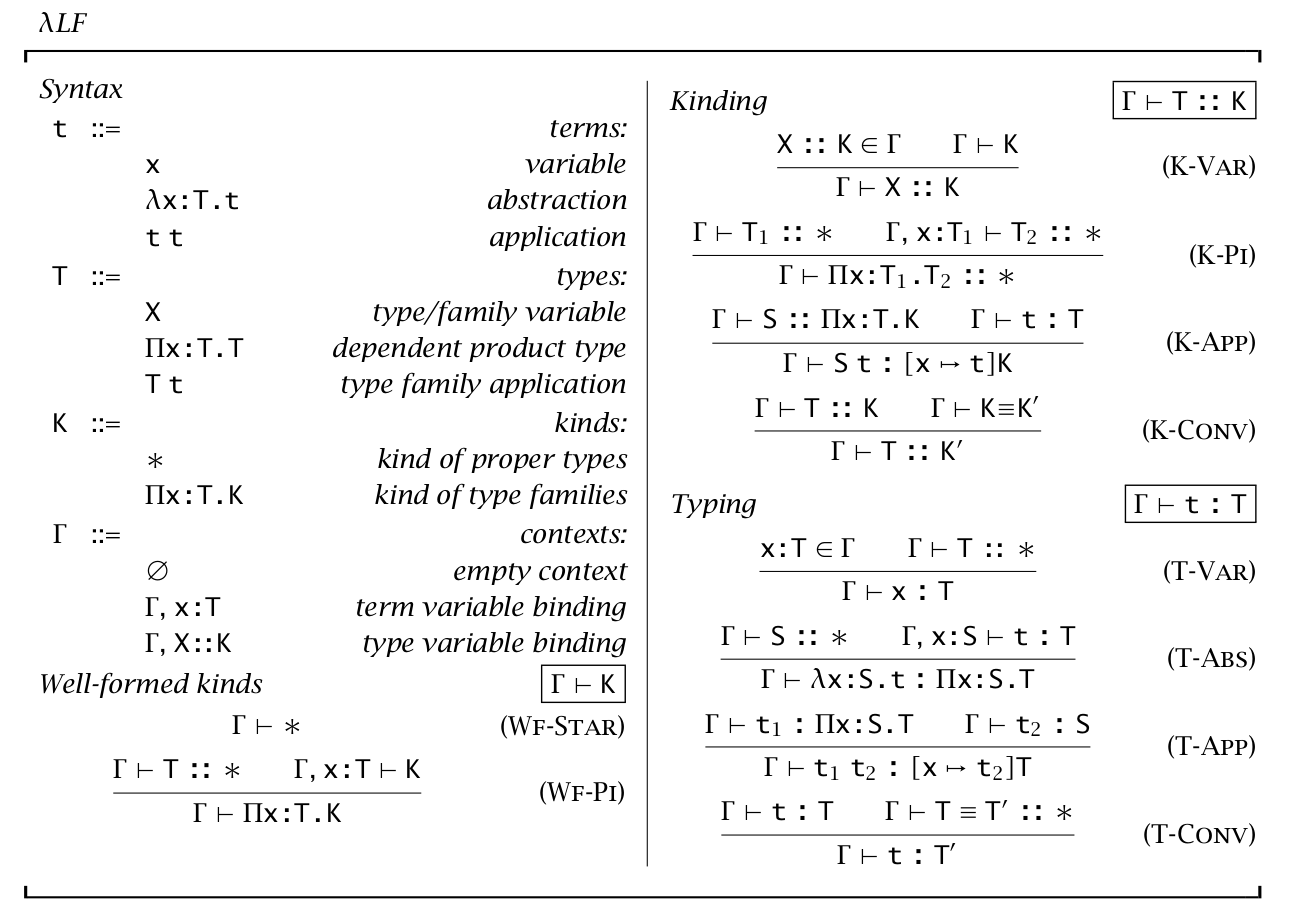
\includegraphics[scale=0.35]{img/lp.png}
	\caption{Язык с лямбдой и $\Pi$-типами }
	\label{lpi}
\end{figure}

В данном нас явно выделяются три сорта (можно думать о сортах как о метатипах): кайнды, термы и типы (правила связанные с кайндами и само их описание опущены для простоты).

Также явно выделяются примитивы языка\footnote{В дальнейшем мы называем их функциональными символами.}:
абстракция, пи-типы (стрелки в языках без зависимых типов) и аппликация. Легко заметить, что во всех яхыках присутствуют подстановка, контексты, символ ':' означающий, что тип терма слева есть терм справа, и связывание переменных.

Правила вида T-Conv и T-Var всегда верны в зависимых языках, поэтому у нас они есть по умолчанию. Также подразумевается рефлексивность, симметричность, транзитивность и конгруэнтность равенства.

Если принять во внимания все наблюдения выше то так этот язык будет выглядеть в нашем языке спецификации\footnote{Важно понимать, что запись $\_ \vdash$ не означает, что контекст пуст, если слева ничего не написано, это эквивалентно записи $\Gamma \vdash$.}:

\begin{lstlisting}
DependentSorts:
  tm, ty
FunctionalSymbols:
  lam: (ty, 0)*(tm, 1) -> tm
  app: (tm, 0)*(tm, 0)*(ty, 1) -> tm
  pi : (ty, 0)*(ty, 1) -> ty
Axioms:
  K-Pi =
    forall T1 : ty, x.T2 : ty
      x : T1 |- T2 def |--- |- pi(T1, x.T2) def

  TAbs =
    forall S : ty, x.T : ty, x.t : tm
      x : S |- t : T |--- |- lam(S, x.t) : pi(S, x.T)
  TApp =
    forall t1 : tm, t2 : tm, S : ty, x.T : ty
            |- t1 : pi(S, x.T),
            |- t2 : S,
      x : S |- T def
      |--------------------------
      |- app(t1, t2, x.T) : T[x:=t2]
Reductions:
  Beta =
    forall x.b : tm, A : ty, a : tm, z.T : ty
       |--- |- app(lam(A, x.b), a, z.T) => b[x:=a] : T[z:=a]

\end{lstlisting}

Типизирование метапеременных позволяет проверять правильность применения функциональных символов и наличие нужных переменных в контексте. Именованные переменные служат для определения порядка переменных в контексте и не несут какой-то дополнительной информации.

Также в язык была добавлена проверка на c-стабильность --- можно помечать аксиомы типами, тогда аксиома применима, только если все переменные входящие в терм являются представителями этих типов\footnote{Если список типов пуст, то производится проверка на отсутствие свободных переменных.}.

\subsection{Ограничения на спецификации, налагаемые языком}

Если рассматривать спецификации как произвольные существенно алгебраические теории, то пользователь может написать спецификацию, для которой мы не сможем сгенерировать тайпчекер. Поэтому вводятся следующие ограничения на спецификации языков:

\begin{enumerate}
\item Запрещено равенство в заключении аксиом для определенности каждого шага в проверке типов определяемого языка Это связано с тем, что, если мы видим равенство, не ясно в какую сторону идти при редуцировании.

\item Если в заключении аксиомы написан функциональный символ возвращающий сорт термов, он обязан также иметь тип (нельзя просто написать $ \vdash f(\ldots) def$). Так как становится неясно какой тип возвращать при выводе типов.

\item Определения функциональных символов всегда одно, иначе появляется недетерминированность в проверке типов. Не играет особой роли, так как в данном случае можно сделать недетерминированность в проверке.

\item Подстановки разрешены только в метапеременные --- в принципе, это слабое ограничение, которое облегчает жизнь при реализации, не ограничивая пользователя.

\item \label{tm:Meta} Все метапеременные используемые в предпосылках должны либо присутствовать в метапеременных заключения или же должны быть типами какой-либо предпосылки. Иначе нужно считать, что это верно для любого представителя сорта метапеременной.

\item Если в функциональном символе встречаются метапеременные с контекстами $x_1 \ldots x_k . T$ должна существовать предпосылка вида $x_1 : S_1 \ldots x_k : S_k  \vdash T$. Это сделано для того чтобы не передавать типы контекстов метапеременных функционального символа явно.

\item Если метапеременная является типом предпосылки и не встречается в аргументах функционального символа, то она может использоваться только справа от двоеточия. Таким образом избегаются ситуации связанные с порядком проверки предпосылок языка. А именно: если у нас есть $x : S \vdash t : T,\ x:T \vdash r : S$, то нужно строить граф зависимостей для предпосылок и использовать порядок полученный в результате его топологической сортировки в генерации кода. (Аналогично с~\ref{toposort}).

\item \label{order:Meta} Все переменные контекстов определения метапеременных могут использовать только метапеременные левее внутри функционального символа в заключении --- это связано с тем, что иначе могут возникнуть циклы в определениях метапеременных: S тип с аргументом типа R, R тип с аргументом типа S, S тип с аргументом типа R...

\item Из-за ослабления условия на метапеременные в Пункте~\ref{tm:Meta}, порядок метапеременных неочевиден. Решение данной проблемы и~(\ref{order:Meta}) описано в Секции~\ref{toposort}.

\item Редукции не учитывают предпосылок при приведении в нормальную форму --- предполагается что они не конфликтуют с аксиомами и проверки в аксиомах достаточно.

\item В редукциях все метапеременные справа от '=>' должны встречаться и слева от него. Иначе непонятно откуда их взять.

\item Подстановка запрещена слева от '=>'.

\item Все редукции всегда стабильны.

\item Все аргументы в функциональный символ в заключении аксиомы должны быть метапеременными --- случай с не только метапеременными требует дальнейшего исследования. Ещё и с теми же аргументами, что и в forall (не расширенный котекст, не существенно).

\item В заключении контекст не должен быть расширен --- это ограничение связано с тем, что иначе смысл аксиомы становится странным. А именно: функциональный символ применим только при введении переменных в контекст.

\end{enumerate}

Также у нашего языка есть ограничения, налагаемые существенно-алгебраическими теориями:
\begin{itemize}
\item Все используемые метапеременные должны иметь аннотацию (сорт), то есть присутствовать в секции forall аксиомы/редукции.
\item Мы явно специфицируем все сорты, которые используем.
\end{itemize}

\subsection{Проверки корректности спецификации языка}

Все ограничения выше проверяются при обработке спецификации языка.

Также тривиальными проверками, осуществляемыми после парсинга языка, являются:
\begin{itemize}
\item Все метапеременные, используемые в правилах вывода/редукциях находятся в контексте включающем их контекст описанный в секции forall.
\item Проверка того, что сорты используемых выражений совпадают с сортами аргументов функциональных символов.
\item Подстановка осуществляется в переменные, которые есть в свободном виде в метапеременной.
\item Контексты метапеременных содержат все их метапеременные.
\item Все функциональные символы имеют ассоциированное правило вывода.
\end{itemize}
